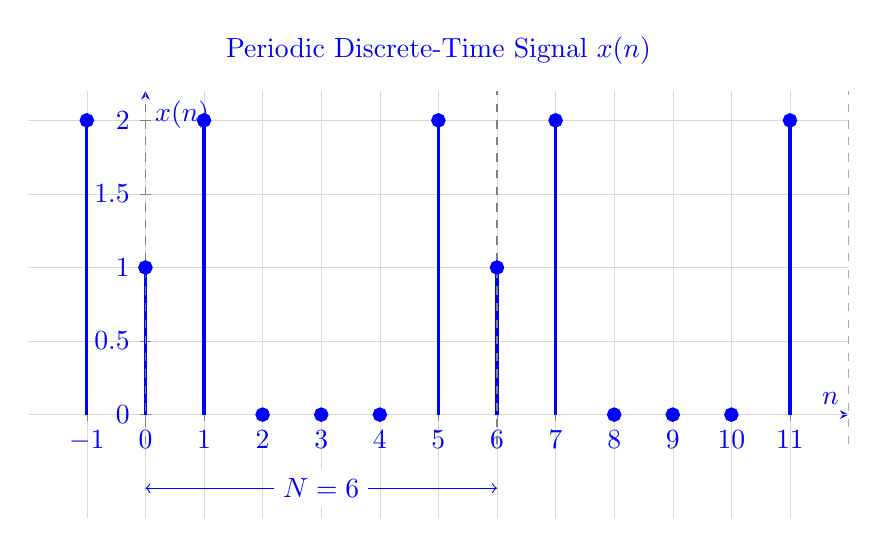
\begin{tikzpicture}
\begin{axis}[
    width=12cm,
    height=7cm,
    axis lines=middle,
    xlabel={$n$},
    ylabel={$x(n)$},
    title={Periodic Discrete-Time Signal $x(n)$},
    xmin=-2, xmax=12,
    ymin=-0.7, ymax=2.2,
    xtick=\empty,
    ytick=\empty,
    extra x ticks={-1, 0, 1, 2, 3, 4, 5, 6, 7, 8, 9, 10, 11},
    extra y ticks={0, 0.5, 1, 1.5, 2},
    grid=major,
    grid style={line width=.1pt, draw=gray!30},
    ycomb, % Discrete-time plot
    mark=*, mark size=2pt, blue,
]

% Plot the periodic discrete-time signal
\addplot[ycomb, blue, very thick, mark=*, mark size=2pt] coordinates {
    (-1, 2) (0, 1) (1, 2) (2, 0) (3, 0) (4, 0) (5, 2) (6, 1) (7, 2) (8, 0) (9, 0) (10, 0) (11, 2)
};

% Add period markers
\draw[dashed, gray] (0, -0.2) -- (0, 2.2);
\draw[dashed, gray] (6, -0.2) -- (6, 2.2);
\draw[dashed, gray] (12, -0.2) -- (12, 2.2);

% Add period label
\draw[<->] (0, -0.5) -- (6, -0.5) node[midway, fill=white] {$N = 6$};

% Add annotation
%\node[anchor=west, fill=white, inner sep=2pt] at (2, 1.5) {Periodic pattern: $[2, 1, 2, 0, 0, 0]$};\\

\

\end{axis}
\end{tikzpicture}
